\documentclass[10pt]{article} % per mettere il fontsize a 10pt
\usepackage{graphicx} % Required for inserting images
\usepackage{array}
\usepackage{longtable}
\usepackage{geometry}
\usepackage{amsmath}
\usepackage{makecell}
\usepackage{xcolor}
\usepackage[table]{xcolor}
\usepackage{color}
\usepackage{amssymb}
\usepackage{soul}
\usepackage{multirow}
\usepackage{booktabs}
\usepackage{float}
\usepackage{comment}
\usepackage{subcaption}
\usepackage{tikz}
\usetikzlibrary{positioning, arrows.meta}
\usepackage{hyperref}
\usepackage [english]{babel}
\addto\captionsenglish{% Replace "english" with the language you use
  \renewcommand{\contentsname}%
    {Table Of Contents}%
}
\usepackage [autostyle, english = american]{csquotes}
\usepackage{changepage}
\MakeOuterQuote{"}
\font\myfontheader=cmcsc10 at 12pt
\font\myfont=cmcsc10 at 16pt
\font\myfonts=cmr12 at 22pt
\font\myfontnames=cmr12 at 12pt
\geometry{
 a4paper,
 total={170mm,257mm},
 left=18mm,
 right=18mm,
 top=26mm,
 bottom=26mm
 }
 
\begin{document}
\pagenumbering{gobble}

\title{
    \includegraphics[width=0.15\textwidth]{img/unipi.png}\\[0.2cm]
    {\myfontheader University of Pisa}\\
    {\myfontheader Department of Computer Science}\\[1.3cm]
    {\myfont Visual Analytics}\\[0.5cm]
    {\myfonts Tracking Suspicious Fishing Activity:\\[0.1cm] 
    Solving the VAST Challenge 2024}
}

\author{
    {\myfontnames Matilde Contestabile}\\[0.1cm]
    {\small Student ID: 639307}\\
    {\small \texttt{m.contestabile1@studenti.unipi.it}}
}
\date{ }

\maketitle

\vspace{1.2cm}

\begin{abstract}
\begin{adjustwidth}{2cm}{2cm}
    This report describes the design and implementation of an interactive visual analytics system developed for the VAST Challenge 2024 (Mini-challenge 2). The system enables exploration of vessel activity and fish transactions, allowing users to identify patterns, anomalies, and potential illegal behavior. We detail the dataset, the analytical approaches applied during exploratory data analysis, and the rationale behind the visual design choices, including color, layout, and interaction strategies. Through dynamic visual representations, the system supports both high-level overviews and detailed investigation, facilitating the discovery of insights and supporting analytical tasks in complex data.

\end{adjustwidth}
\end{abstract}

\vfill % Spinge tutto il resto in fondo
    
\centering
% --- FOOTER ---
\rule{0.8\textwidth}{0.4pt}\\ % Linea orizzontale
\vspace{0.4cm}
\textit{Academic Year 2024/2025}

\begin{adjustwidth}{1cm}{1cm}

% ToC
\newpage
\tableofcontents
\clearpage

\pagenumbering{arabic}
%---------------------------------------------------------------
\section{Introduction}
\subsection{Project Overview and VAST Challenge Context} \label{challenge_context}

This project addresses the analytical goals of the \textbf{Mini-Challenge 2 (MC2)} from the \textbf{VAST Challenge 2024} (available for consultation at \url{https://vast-challenge.github.io/2024/index.html}). The VAST Challenge is a well-established international competition focusing on advanced visual analytics. The 2024 edition is set in the fictional nation of Oceanus, where a vibrant commercial fishing industry is facing threats from unethical practices by certain actors.
The \textit{Challenge Overview} recites as follows:

\begin{quote} \small
    Welcome to Oceanus, an island nation with a healthy market for commercial fishing. Most companies in the region are united in following regulations and implementing sustainable fishing practices. But there are a few companies who are willing to cross ethical lines to increase their catch and their profits. Luckily, FishEye International maintains a watchful eye on fishing data. Their dedicated analysts have been processing data from various sources into a knowledge graph that they call CatchNet: the Oceanus Knowledge Graph.
\end{quote}

In this context, \textbf{Mini-Challenge 2 (MC2)} focuses on analyzing the behavior of vessels operating within Oceanus using multiple datasets, including transponder pings, harbor visit records, and transaction logs. The central goal is to investigate \textbf{illegal fishing behaviors} by the company \textbf{SouthSeafood Express Corp} and to develop visualizations that support \textbf{anomaly detection in vessel movements and supply chains}. Here's the \textit{overview} specific to the mini-challenge:

\begin{quote} \small
    In Oceanus, island life is defined by the coming and going of seafaring vessels, many of which are operated by commercial fishing companies. Typically, the movement of ships and goods are a sign of Oceanus’s healthy economy. But mundane routines can be disrupted by a major event.\vspace{0.3em}

    FishEye International has discovered that SouthSeafood Express Corp was engaged in illegal fishing, prompting the need for advanced analysis. As part of this challenge, analysts must investigate this event using CatchNet data to uncover behavioral patterns, track fish product movements, and support future monitoring.
\end{quote}

More specifically, the mini-challenge requires to address the following research questions through a series of targeted visual workflows and analytical strategies, with an emphasis on interactivity and clarity:

\begin{enumerate}
    \item \textbf{Cargo Attribution:} Given the lack of direct vessel identifiers in port transaction records (due to wrong purchase of records by FishEye analysts), can we visually and analytically associate cargo deliveries with specific vessels? What seasonal or regional trends emerge in fish exports?

    \item \textbf{Illegal Behavior Detection:} How do the trajectories and port interactions of SouthSeafood Express vessels differ from compliant vessels? When and where did violations occur?

    \item \textbf{Behavioral Pattern Matching:} Are there other vessels whose behavior mirrors that of SouthSeafood Express? Can similar illegal activities be inferred?

    \item \textbf{Post-Incident Trends:} Following the discovery of illegal fishing, have commercial fishing patterns across Oceanus shifted? Are new anomalies emerging?
\end{enumerate}

Answers are available at Section~\ref{research-questions}.

%---------------------------------------------------------------
\subsection{Repository and Resources}

The full implementation is publicly available in the GitHub repository:
\begin{quote}
\url{https://github.com/matildeec/VisualAnalytics2025}
\end{quote}

The repository includes:
\begin{itemize}
    \item \texttt{data-understanding/} – Notebook-based data inspection and cleaning scripts
    \item \texttt{platform/} – Visualization platform built with D3.js and Altair
    \item \texttt{notebooks/} – Exploratory and analytical notebooks addressing each research question
    \item \texttt{data/} – Cleaned and raw JSON graph files
\end{itemize}

To install, clone the repository and install the required dependencies:

\begin{verbatim}
git clone https://github.com/matildeec/VisualAnalytics2025.git
cd VisualAnalytics2025
pip install -r requirements.txt
\end{verbatim}

\noindent The project is fully reproducible and structured for modular exploration and extension.

\section{Data Understanding and Preprocessing}

This section outlines the data exploration and cleaning process carried out for the VAST Challenge 2024 Mini-Challenge 2. Using a data mining approach and Python libraries, we prepared the knowledge graph dataset for visual exploration and anomaly detection, specifically, in a format suitable for JavaScript-based applications.

\subsection{Data Sources and File Structure}

The challenge dataset consists of multiple files, with the central one being a JSON-encoded knowledge graph representing vessel activities, harbor transactions, and commercial fishing behaviors. Supplementary files provide metadata and geospatial context.

\begin{table}[h!]
\centering
\small
\begin{tabular}{p{5.2cm}p{8.8cm}}
\hline
\textbf{File Name} & \textbf{Description} \\
\hline
\texttt{mc2.json} & Main knowledge graph, structured as a multigraph with typed nodes and edges representing entities and events (e.g., vessels, ports, transactions, pings). \\
\hline
\texttt{Oceanus Geography Nodes.json} & Metadata for geographic locations (e.g., ports, reefs, regions). \\
\hline
\texttt{Oceanus Geography.geojson} & Geospatial file for mapping entities in Oceanus. \\
\hline
\end{tabular}
\caption{Overview of provided data files}
\end{table}

To support understanding of the knowledge graph, the document \texttt{VAST2024 - MC2 Data Description.docx} is provided, detailing the graph structure and entity semantics.

\subsection{Graph Structure Analysis and Preprocessing}

The knowledge graph contained in \texttt{mc2.json} was imported using the \texttt{networkx} library, resulting in a directed multigraph. Nodes and edges include a \texttt{type} attribute, which was used to categorize and filter graph elements. Both nodes and edges were extracted into separate Pandas DataFrames to enable structured analysis.

Initial preprocessing involved removing metadata fields irrelevant to downstream analysis, specifically: \texttt{[\_last\_edited\_by, \_last\_edited\_date, \_date\_added, \_raw\_source, \_algorithm]}. 

Next, nodes (entities) and edges (events) were grouped by their \texttt{type}. Within each group, columns containing only missing values were discarded, and only relevant attributes were retained to support visualization and modeling tasks.

A summary table of the cleaned data files intended for use in the JavaScript implementation is provided at the end of this section.

\subsubsection{Node Overview and Distribution}

The knowledge graph contains a diverse set of node types. Table~\ref{tab:nodes} summarizes the most relevant node types by category, showing the number of instances and representative attributes retained after cleaning.

{ \small
\begin{longtable}{@{}l >{\raggedright\arraybackslash}p{5.2cm} c >{\raggedright\arraybackslash}p{6.2cm}@{}}
\caption{Updated Node Types with Attributes in the Knowledge Graph} \label{tab:nodes} \\

% --- Header first page ---
\toprule
\textbf{Category} & \textbf{Node Type} & \textbf{Count} & \textbf{Attributes} \\
\midrule
\endfirsthead

% --- Header following pages ---
\caption[]{Updated Node Types with Attributes in the Knowledge Graph} \\
\toprule
\textbf{Category} & \textbf{Node Type} & \textbf{Count} & \textbf{Attributes} \\
\midrule
\endhead

\midrule
\multicolumn{4}{r}{\textit{Continued on next page...}} \\
\endfoot

\bottomrule
\endlastfoot

% --- Table content ---
Document
  & Entity.Document.DeliveryReport & 5307 & \texttt{qty\_tons}, \texttt{date} \\
\midrule

\multirow{7}{*}{Vessel}
  & Entity.Vessel.FishingVessel     & 178 & \texttt{name}, \texttt{flag\_country}, \texttt{company}, \texttt{tonnage}, \texttt{length\_overall} \\
  & Entity.Vessel.CargoVessel       & 100 & \texttt{name}, \texttt{flag\_country}, \texttt{company}, \texttt{tonnage}, \texttt{length\_overall} \\
  & Entity.Vessel.Ferry.Passenger   & 3   & \texttt{name}, \texttt{flag\_country} \\
  & Entity.Vessel.Ferry.Cargo       & 2   & \texttt{name}, \texttt{flag\_country} \\
  & Entity.Vessel.Tour              & 6   & \texttt{name}, \texttt{flag\_country} \\
  & Entity.Vessel.Research          & 2   & \texttt{name}, \texttt{flag\_country} \\
  & Entity.Vessel.Other             & 5   & \texttt{name}, \texttt{flag\_country}, \texttt{length\_overall} \\
\midrule

\multirow{3}{*}{Location}
  & Entity.Location.Point           & 12  & \texttt{name}, \texttt{description}, \texttt{activities}, \texttt{kind} \\
  & Entity.Location.City            & 6   & \texttt{name}, \texttt{activities}, \texttt{kind} \\
  & Entity.Location.Region          & 6   & \texttt{name}, \texttt{description}, \texttt{activities}, \texttt{kind}, \texttt{fish\_species\_present} \\
\midrule

Commodity
  & Entity.Commodity.Fish           & 10  & \texttt{name} \\

\end{longtable}
}

\subsubsection{Edge Types and Event Semantics}

Edges in the knowledge graph represent interactions and events between entities, providing both temporal and relational context to the data. Table~\ref{tab:edges} summarizes the original edge types, including their counts, source and target entities, and retained attributes.

% \textbf{Event.TransportEvent.TransponderPing} edges capture vessel GPS signals, including timestamps and dwell times, enabling us to reconstruct vessel movement patterns;  
% \textbf{Event.HarborReport} edges represent port activity recorded by portmasters, including vessel arrivals and departures;  
% \textbf{Event.Transaction} edges describe seafood deliveries to specific locations and link delivery reports to the commodities they contain.

\begin{table}[H]
\centering
\small
\renewcommand{\arraystretch}{1.15}
\setlength{\tabcolsep}{6pt}
\begin{tabular}{@{}>{\raggedright\arraybackslash}p{5.5cm} c >{\raggedright\arraybackslash}p{2.2cm} >{\raggedright\arraybackslash}p{2.4cm} >{\raggedright\arraybackslash}p{2.8cm}@{}}
\toprule
\textbf{Event Type} & \textbf{Count} & \textbf{Source} & \textbf{Target} & \textbf{Attributes} \\
\midrule
Event.TransportEvent.TransponderPing & 258,542 & Entity.Location & Entity.Vessel & \texttt{time}, \texttt{dwell} \\
Event.Transaction                     & 5,307  & Entity.Document & Entity.Commodity & \texttt{date} \\
Event.Transaction                     & 5,307  & Entity.Document & Entity.Location & \texttt{date} \\
Event.HarborReport                   & 2,487  & Entity.Vessel  & Entity.Location  & \texttt{date}, \texttt{data\_author} \\
\bottomrule
\end{tabular}
\caption{Original edge types with counts, sources, targets, and attributes.}
\label{tab:edges}
\end{table}

From here, two critical issues become apparent that affect readability and understanding of the data.  
First, for \textbf{Event.HarborReport}, the edge direction is counterintuitive: while the information originates from portmasters, the current structure connects vessels (sources) to ports (targets). Reversing this direction would better reflect data provenance and better match with \textbf{Event.TransportEvent. \allowbreak TransponderPing}.  
Second, \textbf{Event.Transaction} edges are redundant: each delivery report is linked to both a location and a commodity via two separate edges, resulting in duplication and unnecessary complexity.

To address these issues, we redesigned the schema. Information about commodities, including species and quantities, has been moved into the delivery report entity itself, while \textbf{Event.Transaction} edges now exclusively connect delivery reports (sources) to locations (targets).  
The updated structure is summarized in Table~\ref{tab:edges-redesigned}.

\begin{table}[H]
\centering
\small
\renewcommand{\arraystretch}{1.15}
\setlength{\tabcolsep}{6pt}
\begin{tabular}{@{}>{\raggedright\arraybackslash}p{5.5cm} c >{\raggedright\arraybackslash}p{2.2cm} >{\raggedright\arraybackslash}p{2.4cm} >{\raggedright\arraybackslash}p{2.8cm}@{}}
\toprule
\textbf{Event Type} & \textbf{Count} & \textbf{Source} & \textbf{Target} & \textbf{Attributes} \\
\midrule
Event.TransportEvent.TransponderPing & 258,542 & Entity.Location & Entity.Vessel & \texttt{time}, \texttt{dwell} \\
Event.Transaction                    & 5,307  & Entity.Document & Entity.Location & \texttt{date} \\
Event.HarborReport                  & 2,487  & Entity.Location & Entity.Vessel  & \texttt{date}, \texttt{data\_author} \\
\bottomrule
\end{tabular}
\caption{Updated edge types}
\label{tab:edges-redesigned}
\end{table}

\subsubsection{Cargo Attribution via Suspected Vessels Tagging}

To address the challenge of associating cargo deliveries with specific vessels despite missing direct identifiers in the port transaction records (see Question 1 in \ref{challenge_context}), we introduced an attribute called \texttt{suspected\_vessels} within the transactions dataset which was derived in an analytical way. This attribute records, for each transaction, a list of vessels potentially responsible for the cargo. The goal was to infer likely vessel–cargo associations based on spatiotemporal docking information and the presence of fish species in regions. The logic underlying this inference can be formalized as:
{\small
\[
\begin{aligned}
& \textit{Vessel is either `CargoVessel', `FishingVessel' or `Other' } \\
& \wedge\ \textit{Vessel is docked in a harbor where a fish species was exported (within 1 day)} \\
& \wedge\; \textit{The same species is present in a region earlier visited by the vessel} \\
& \implies \textit{The fish species is likely the vessel's cargo.}
\end{aligned}
\]
}

Applying this rule, we flagged transactions meeting these conditions and annotated them with the corresponding \texttt{suspected\_vessels}. A visual summary of the logic is provided in Figure~\ref{fig:suspected_vessels_flowchart}.

\begin{figure}[h!]
\centering
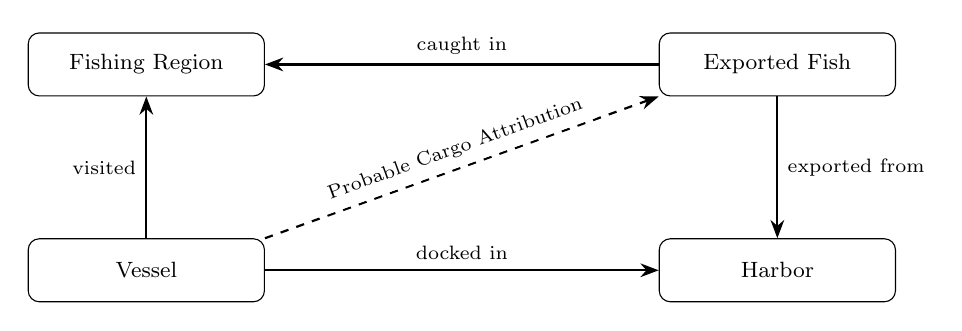
\begin{tikzpicture}[
  node/.style={draw, rounded corners, align=center, minimum width=3cm, minimum height=0.8cm, font=\footnotesize},
  arrow/.style={-{Stealth[scale=1]}, thick},
  inferred/.style={-{Stealth[scale=1]}, thick, dashed},
  node distance=1.8cm and 5cm
]

% Nodes
\node[node] (fish) {Exported Fish};
\node[node, below=of fish] (harbor) {Harbor};
\node[node, left=of harbor] (vessel) {Vessel};
\node[node, above=of vessel] (region) {Fishing Region};

% Arrows with plain text labels
\draw[arrow] (fish) -- (harbor) node[midway, right, font=\scriptsize, fill=white]{exported from};
\draw[arrow] (fish) -- (region) node[midway, sloped, above, font=\scriptsize, fill=white]{caught in};
\draw[arrow] (vessel) -- (harbor) node[midway, above, font=\scriptsize, fill=white]{docked in};
\draw[arrow] (vessel) -- (region) node[midway, left, font=\scriptsize, fill=white]{visited};

% Inferred diagonal arrow with plain text
\draw[inferred] (vessel.north east) -- (fish.south west) 
  node[midway, sloped, above, font=\scriptsize, fill=white]{Probable Cargo Attribution};

\end{tikzpicture}
\caption{
Flowchart showing derivation of the \texttt{suspected\_vessels} attribute.
}
\label{fig:suspected_vessels_flowchart}
\end{figure}

\subsection{Resulting \texttt{.json} Files}

Table~\ref{tab:cleaned-json-files} summarizes the cleaned and structured \texttt{.json} files generated from the original knowledge graph after preprocessing. These files are optimized for use in the JavaScript-based implementation and support efficient querying since together they construct a database with primary (underlined) and foreign keys.

\begin{table}[H]
\centering
\small
\renewcommand{\arraystretch}{1.15}
\setlength{\tabcolsep}{6pt}
\begin{tabular}{@{}>{\raggedright\arraybackslash}p{3.6cm} >{\raggedright\arraybackslash}p{2.6cm} >{\raggedright\arraybackslash}p{7.7cm}@{}}
\toprule
\textbf{File Name} & \textbf{Description} & \textbf{Keys} \\
\midrule
\texttt{vessels.json}           & Vessel entities        & \underline{\texttt{id}}, \texttt{vessel\_type}, \texttt{name}, \texttt{company}, \texttt{flag\_country}, \texttt{tonnage}, \texttt{length\_overall} \\
\texttt{commodities.json}       & Traded fish            & \underline{\texttt{id}}, \texttt{name} \\
\texttt{documents.json}         & Delivery reports       & \underline{\texttt{id}}, \texttt{commodity}, \texttt{qty\_tons} \\
\texttt{locations.json}         & Locations & \underline{\texttt{id}}, \texttt{name}, \texttt{location\_type}, \texttt{kind}, \texttt{description}, \texttt{activities}, \texttt{fish\_species\_present} \\
\texttt{transponder\_pings.json} & Vessel GPS logs       & \underline{\texttt{source}}, \underline{\texttt{target}}, \texttt{time}, \texttt{dwell} \\
\texttt{harbor\_reports.json}   & Port-exit records     & \underline{\texttt{source}}, \underline{\texttt{target}}, \texttt{date}, \texttt{data\_author} \\
\texttt{transactions.json}      & Cargo exchanges        & \underline{\texttt{source}}, \underline{\texttt{target}}, \texttt{date}, \texttt{suspected\_vessels} \\
\bottomrule
\end{tabular}
\caption{Cleaned \texttt{.json} files and their key attributes. Underlined keys indicate primary identifiers.}
\label{tab:cleaned-json-files}
\end{table}

To further facilitate the representation of vessel trajectories, a dedicated file named \texttt{trajectories.json} was created. It is structured as a dictionary, where the keys are vessel IDs and the values are ordered lists of transponder pings represented as JSON objects.
\section{Exploratory Data Analysis} \label{eda}

We conducted an initial exploratory data analysis (EDA) on the cleaned data using a combination of Python libraries such as \texttt{pandas}, \texttt{matplotlib}, \texttt{altair}, and \texttt{seaborn}. The purpose of this analysis was to uncover patterns in vessel activity, identify potential anomalies, and provide a foundation for more sophisticated visualizations later on.

\subsection{Analytical Analysis of vessel activity}

To effectively interpret vessel behavior, it was first necessary to understand the geographical context of the dataset. Certain regions are in fact designated as ecological preserves, where fishing activity is strictly prohibited. Vessels, however, were observed operating across both legal fishing grounds and these protected zones. Additionally, the dataset provides the list of species present in every region, allowing us to identify which species are exclusive to protected preserves. Using this information, we derived an analytical classification of \emph{illegal species}, defined as those found exclusively within protected preserves, and \emph{suspect} ones, which appear in both legal and illegal zones. Table~\ref{tab:species-matrix} summarizes this mapping: species highlighted in red appear only in illegal zones and therefore serve as indicators of potential illegal fishing activity, while those in yellow are considered suspect due to their presence in both legal and illegal areas. 

\begin{table}[H]
\centering
\footnotesize
\setlength{\tabcolsep}{4pt}       % reduce horizontal padding
\renewcommand{\arraystretch}{0.95} % tighter rows
\begin{tabular}{|l|c c c|>{\columncolor{red!5}}c|>{\columncolor{red!5}}c|>{\columncolor{red!5}}c|}
\hline
\textbf{Fish Species} & Cod Table & Wrasse Beds & Tuna Shelf & Ghoti Preserve & Nemo Reef & Don Limpet Preserve \\ \hline
\texttt{gadusnspecificatae4ba}   & \checkmark &  &  &  &  &  \\ \hline
\rowcolor{yellow!15} \texttt{piscesfrigus900}         & \checkmark & \checkmark & \checkmark &  & \checkmark & \checkmark \\ \hline
\rowcolor{yellow!15} \texttt{habeaspisces4eb}         & \checkmark & \checkmark & \checkmark & \checkmark & \checkmark & \checkmark \\ \hline
\rowcolor{yellow!15} \texttt{labridaenrefert9be}      &  & \checkmark &  & \checkmark & \checkmark &  \\ \hline
\rowcolor{red!15} \texttt{piscessatisb87}   &  &  &  & \checkmark & \checkmark & \checkmark \\ \hline
\rowcolor{red!15} \texttt{piscisosseusb6d}  &  &  &  & \checkmark &  &  \\ \hline
\rowcolor{yellow!15} \texttt{thunnininveradb7}        &  &  & \checkmark &  & \checkmark & \checkmark \\ \hline
\rowcolor{red!15} \texttt{piscesfoetidaae7} &  &  &  &  &  & \checkmark \\ \hline
\texttt{piscissapidum9b7}        &  &  & \checkmark &  &  &  \\ \hline
\end{tabular}
\caption{Matrix of fish species presence across regions. Rows in red indicate species found exclusively in ecological preserves (illegal). Shaded columns mark the illegal fishing zones.}
\label{tab:species-matrix}
\end{table}

After establishing a clear mapping of legal versus illegal zones and species, we turned our attention to temporal patterns in vessel behavior. Specifically, we examined three features: \emph{dwell time} (how long a vessel remained near a given location), \emph{gaps between transponder pings}, and \emph{harbor visit frequencies}.

The rationale was straightforward. Prolonged dwell times may signal suspicious activity, such as covert fishing or offloading. Unusual gaps in transponder signals could indicate attempts at evasion, while irregular harbor visits might point to atypical supply or unloading patterns.

\begin{figure}[H]
    \centering
    \includegraphics[width=0.8\linewidth]{img/dwell-by-location.png}
    \caption{Dwell time of fishing vessels by location.}
    \label{fig:dwell-by-location}
\end{figure}

Of these features, however, the latter two proved less reliable as standalone indicators. Coverage gaps were common but did not consistently align with illegal fishing zones, and variations in harbor visit frequency were not necessarily suspicious when taken in isolation. By contrast, the dwell time analysis provided the clearest signals of anomalous vessel behavior and thus emerged as the most informative exploratory measure. Figure~\ref{fig:dwell-by-location} illustrates these dwell time patterns across different locations.

The boxplots make clear that vessels indeed lingered significantly longer at certain locations than expected. While many values fell within a normal operational range, some extreme outliers stand out and warrant further investigation. This insight guided the direction of subsequent visualizations, where the emphasis shifted toward tracking how vessels move, where they pause, and how these behaviors align with known illegal regions.


\subsection{Temporal Analysis of Fish Deliveries}
To better grasp the scale of fish deliveries, we aggregated transaction records to track quantities over time. This allowed us to identify seasonal dynamics, peak transaction periods, and potential export trends as requested in Q1. Figure~\ref{fig:transaction-volume} illustrates total transaction volumes for South Paackland as an example case. Noticeable spikes suggest periods of heightened demand, which may align with peak fishing activity or, in some cases, potential illegal operations.

In the visualization, illegal fish species are highlighted in shades of red, while legal (including suspect) species are shown in shades of blue, enabling a direct comparison of their relative contribution to overall trade flows. This perspective not only informed our analysis but also shaped the subsequent design of our visualization approach.

\begin{figure}[h]
    \centering
    \includegraphics[width=0.9\linewidth]{img/imports_1.png}
    \caption{Transaction volume over time, representing fish deliveries. Illegal species are shown in shades of red, while legal species are shown in shades of blue.}
    \label{fig:transaction-volume}
\end{figure}

\subsection{Analytical Analysis of SouthSeafood Express Corp vessels}

As part of our EDA, we conducted a focused investigation of the company identified as engaging in illegal activities, \textit{SouthSeafood Express Corp}, as requested by the challenge. Table~\ref{tab:southseafood} summarizes the two vessels associated with this company, including their vessel IDs, names, and tonnage.

\begin{table}[H]
\centering
\small
\begin{tabular}{lll}
\textbf{Vessel ID} & \textbf{Name} & \textbf{Tonnage} \\
\hline
snappersnatcher7be & Snapper Snatcher & 100 \\
roachrobberdb6     & Roach Robber     & 11,700 \\
\end{tabular}
\caption{Vessels associated with SouthSeafood Express Corp.}
\label{tab:southseafood}
\end{table}

Both vessels were carefully examined for unusual patterns in their activity, including extended dwell times, abnormal harbor visit frequency, and irregular transaction volumes. 

We first established the timeframe of activity prior to the discovery of illegal behavior: \textit{SouthSeafood Express Corp} vessel pings ranged from \texttt{2035-02-01} to \texttt{2035-05-14}. This period serves as a reference for analyzing changes in behavior, relevant to questions such as those in Q4 regarding post-incident trends: whether commercial fishing patterns across Oceanus have shifted and whether new anomalies are emerging.

To assess whether dwell time and other features are indicative of illegal activity, we generated rankings of top dwellers, vessels with the longest ping gaps, and other relevant metrics. In the ranking of dwell times at illegal locations, \texttt{snappersnatcher7be} (Snapper Snatcher) ranked 76th, while \texttt{roachrobberdb6} (Roach Robber) did not appear among the top vessels. This suggests that although Snapper Snatcher spent time at potentially suspicious locations, it was not among the vessels with the longest dwell times, indicating that further analysis is required to determine whether this behavior is significant.  

Similarly, in the analysis of ping gaps, Snapper Snatcher ranked 173rd and Roach Robber 175th. Neither vessel exhibited substantial gaps in their transponder signals, implying that ping gaps alone are not a reliable indicator of evasion or suspicious activity in this context.  

More interesting insights emerged from examining vessel routes based on transponder pings. Snapper Snatcher made multiple visits to \textit{Exit East}, a region designated for deep-sea fishing. While this does not immediately stand out compared to general vessel activity, it raises questions about whether this route reflects typical operational behavior or unusual activity. Further investigation, particularly with complete route visualizations, will help clarify these patterns.  

While detailed considerations of vessel behavior will be presented later as the full visualizations are presented, we provide the initial plot that was generated using Altair to explore these routes.

\begin{figure}[H]
    \centering
    \includegraphics[width=0.9\linewidth]{img/snappersnatcher7be.png}
    \caption{Route of \texttt{Snapper Snatcher}}
    \label{fig:snappersnatcher7be}
\end{figure}

\section{Design and Architecture of the Visual Analytics Interface}

%\url{https://data.europa.eu/apps/data-visualisation-guide/}

The visual analytics interface was designed to support anomaly detection, pattern recognition, and hypothesis generation with the ultimate goal of answering the four research questions reported in Section~\ref{challenge_context}. Guided by established principles of visual encoding, interaction design, and narrative visualization\footnote{Wilke, C. (2019). \textit{Fundamentals of Data Visualization}. Available at \url{https://clauswilke.com/dataviz/}}, the design process consisted of three main stages.
First, we surveyed the state-of-the-art tools to gain inspiration for tracking fishing vessels. Next, we identified the key visual variables necessary to address the research questions posed by the VAST Challenge. Finally, these design decisions were translated into a prototype using Figma, which then served as the blueprint for the implementation of the interactive system in JavaScript.

This section provides a detailed account of the resulting design choices for the visual analytics system developed. 

\subsection{State-of-the-Art Interfaces}

To first gain inspiration, we explored existing platforms addressing similar challenges:

\begin{itemize}
    \item \textbf{VesselFinder}\footnote{Available at \url{https://www.vesselfinder.com/}}: a real-time vessel tracking platform that visualizes vessel locations worldwide using AIS data, providing an intuitive overview of maritime activity.
    \item \textbf{GlobalFishingWatch}\footnote{Available at \url{https://globalfishingwatch.org/map}}: a platform for visualizing global fishing activity, allowing users to monitor vessel movements and identify potential illegal fishing operations.
\end{itemize}

These platforms shaped our initial thinking, particularly in how vessel routes could be represented on a geographic map. However, the structure of our dataset imposed important constraints that made it impossible to reproduce the same level of detailed route visualizations. Although we had geographic coordinates available to reconstruct a map of Oceanus (via the provided \texttt{.geojson} file of Oceanus), the vessel GPS pings did not form a continuous trajectory. Instead, they resembled a series of discrete points – often multiple pings from the same location – linked only by timestamps and dwell times. As a result, we lacked the granular path data necessary to accurately reconstruct “real ocean routes” between locations \textit{A, B}, and \textit{C}.

Rather than forcing an incomplete or misleading geographic reconstruction of exact travel paths, we chose to design visualizations conceptually similar to the static plots created in our Jupyter Notebooks as part of EDA (see Section~\ref{eda}), focusing on patterns and trends in vessel pings – such as timing, frequency, and distribution. This approach allowed us to emphasize meaningful behavioral patterns over potentially inaccurate (and ultimately insignificant) geographic details.

\subsection{Interface Structure and Pattern to Communicate}

To manage the complexity of the data and the multi-faceted research questions, we adopted a multi-page architecture. The application is structured into three distinct views: \textbf{Traffic Explorer}, \textbf{Harbor Activity}, and \textbf{Compare Trajectories}. Each view serves a distinct stage in the analytical pipeline, progressively revealing deeper insights. We provide a brief overview of each page below.

As a design choice, we adopted a \textbf{reader-driven narrative visualization} paradigm, empowering users to explore data at their own pace while providing \textbf{author-driven} entry points (such as pre-selected filters for known violators like SouthSeafood Express Corp) to jumpstart the investigation.

A consistent global navigation bar allows seamless switching between views. To support deep investigation, the interface integrates interactive techniques including zooming, brushing, and "details-on-demand" tooltips, enabling micro-level analysis without cluttering the macro-level visualizations.

\subsubsection{Traffic Explorer}

The \textbf{Traffic Explorer} serves as the primary entry point. It fulfills a dual purpose: establishing geographical context via an \textbf{Interactive Map} and visualizing temporal patterns via a \textbf{Traffic Activity Chart}. This combination allows users to identify macroscopic anomalies in traffic density and spatial distribution.

\paragraph{Interactive Map.}
The spatial component renders the geography of Oceanus using Leaflet and the provided GeoJSON data. It visually distinguishes between functional areas, such as Ecological Preserves (green), Fishing Zones (blue), and landmasses (brown). 

To assist in understanding the complex regulations of the region, the map is linked to a dynamic \textbf{Info Panel}. When a user selects a zone (e.g., \emph{Nemo Reef}), it turns ocre to indicate selection, and the panel populates with semantic metadata, including the zone type, permitted activities (e.g., Recreation, Tourism), and a list of endemic species. This context is critical for identifying illegal fishing activities in protected waters.

\begin{figure}[H]
    \centering
    \begin{subfigure}[b]{0.48\textwidth}
        \centering
        \includegraphics[width=0.6\linewidth, trim=0 9cm 0 0, clip]{img/map_infobox.png}
        \caption{Interactive Map}
        \label{fig:map}
    \end{subfigure}
    \hfill
    \begin{subfigure}[b]{0.48\textwidth}
        \centering
        \includegraphics[width=\linewidth, trim=0 0 0 18cm, clip]{img/map_infobox.png}
        \caption{Info Panel showing zone details}
        \label{fig:chart}
    \end{subfigure}
    
    \caption{The interactive map.}
    \label{fig:traffic_explorer}
\end{figure}

\paragraph{Traffic Activity Chart.}
Upon selecting a zone, the application generates a \textbf{temporal strip plot} to visualize vessel presence over the entire dataset duration (March through November). In this visualization:
\begin{itemize}
    \item The \textbf{Y-axis} lists individual vessels.
    \item The \textbf{X-axis} represents the timeline.
    \item \textbf{Vertical bars} represent discrete "pings" or presence events within the selected zone.
\end{itemize}

Visually resembling a barcode, this density strip allows investigators to instantly recognize patterns, such as regular entry intervals or continuous loitering. 

The chart is equipped with robust filtering capabilities:
\begin{itemize}
    \item \textbf{Time-of-Day Filtering:} Recognizing that illicit activity often occurs during specific windows, a range slider allows users to filter pings by time of day (00:00--24:00). Presets for \emph{Morning}, \emph{Day}, and \emph{Night} allow for rapid comparison of diurnal vs. nocturnal traffic.
    \item \textbf{Visual Highlighting:} To aid the narrative, vessels belonging to \emph{SouthSeafood Express Corp} are highlighted in orange by default, contrasting with the blue of general traffic.
    \item \textbf{Pinning:} Users can "pin" specific vessels of interest, isolating their trajectories for a focused comparison against background traffic noise.
\end{itemize}

\begin{figure}[H]
    \centering
    \includegraphics[width=0.8\linewidth]{img/traffic_chart.png}
    \caption{The Traffic Activity Chart.}
    \label{fig:traffic_chart}
\end{figure}

\subsubsection{Harbor Activity}

The \textbf{Harbor Activity} page focuses on port dynamics, enabling users to analyze cargo exports and harbor visits by specific location. This view is designed to address the core challenge of cargo attribution, which directly addresses Q1. To achieve this, we developed a composite \textbf{Dual-Axis Mirror Plot}, which visually correlates the volume of exports with vessel arrival dynamics on a shared temporal axis.

\paragraph{Data Filtering.}
To manage the high data volume, users can filter cargo by species and vessels by type. Harbors, species.

\begin{figure}[H]
    \centering
    \begin{subfigure}[b]{\textwidth}
        \centering
        \includegraphics[width=0.4\linewidth]{img/harbor_select.png}
        \caption{Harbor selection panel.}
        \label{fig:map}
    \end{subfigure}
    \hfill
    \begin{subfigure}[b]{\textwidth}
        \centering
        \includegraphics[width=0.9\linewidth]{img/filter_panel.png}
        \caption{Filter panel.}
        \label{fig:chart}
    \end{subfigure}
    
    \caption{Harbor selection and filtering panels.}
    \label{fig:filtering_harbor_activity}
\end{figure}

\paragraph{The Mirror Plot.}
This central visualization serves as the analytical engine of the view, split into two aligned components that share a common time axis:
\begin{itemize}
    \item \textbf{Exported Cargo (Top Half):} A \textbf{stacked bar chart} represents the daily volume of fish exports (in tons), color-coded by legal status of species. This allows analysts to instantly detect seasonal anomalies and peaks in illegal shipments.
    \item \textbf{Docked Vessels (Bottom Half):} An \textbf{inverted lollipop chart} visualizes vessel arrivals by gross tonnage (GT) over time. Vessels are colored by type, and the dataset is filtered to include only vessels with registered gross tonnage ($>0$) to focus the analysis on significant maritime activity.
\end{itemize}
By vertically aligning these two datasets, the user can perform visual correlation: a spike in illegal cargo in the top chart can be vertically traced down to identify which heavy-tonnage vessels docked immediately prior to the export. Those analytically linked to illegal shipments are highlighted in red.

\begin{figure}[H]
    \centering
    \includegraphics[width=0.8\linewidth]{img/mirror-plot.png}
    \caption{The Mirror Plot.}
    \label{fig:harbor_overview}
\end{figure}

\paragraph{Interactive Filtering and Suspect Identification.}
To move from visual correlation to specific attribution, the interface employs a \textbf{temporal brushing} interaction. Selecting a time window on the chart updates the \textbf{Details Sidebar}, which lists:
\begin{enumerate}
    \item \textbf{Cargo in Range:} A list of all shipments during the brushed period. Illegal shipments are explicitly flagged with a warning icon (see Figure \ref{fig:sidebar}).
    \item \textbf{Suspect Generation:} Expanding a specific illegal cargo entry reveals a computed list of \textbf{``suspected vessels''} (ships that were docked in the harbor within a relevant time window of the export).
    \item \textbf{Vessels in Range:} A comprehensive list of potential carriers, providing details such as ownership and exact tonnage.
\end{enumerate}

To guide the user's attention, vessels confirmed to be involved in suspicious patterns are highlighted with \textbf{red circles} in the lollipop chart (see Figure \ref{fig:harbor_overview}, bottom right), differentiating them from benign traffic.

\begin{figure}[H]
    \centering
    \begin{subfigure}[b]{0.48\textwidth}
        \centering
        \includegraphics[width=0.5\linewidth]{img/sidebar.png}
        \caption{The Harbor Activity Mirror Plot with the Details Sidebar closed.}
        \label{fig:sidebar_closed}
    \end{subfigure}
    \hfill
    \begin{subfigure}[b]{0.48\textwidth}
        \centering
        \includegraphics[width=0.5\linewidth]{img/sidebar_open.png}
        \caption{The Attribution Sidebar showing suspected vessels for an illegal cargo.}
        \label{fig:sidebar_open}
    \end{subfigure}
    
    \caption{The Attribution Sidebar.}
    \label{fig:sidebar}
\end{figure}

\subsubsection{Compare Trajectories}

Finally, the \textbf{Compare Trajectories} page enables granular comparisons between specific vessel trajectories, addressing Q2 and Q3, about illegal behavior detection and pattern matching. This view consists of a juxtaposed layout, allowing users to select any two vessels via distinct control panels and visualize their movements side-by-side.

\paragraph{Vessel select.}

The vessel selection panels allow users to filter the fleet by company, type, and tonnage range. 

\begin{figure}[H]
    \centering
    \includegraphics[width=0.6\linewidth]{img/vessel_select.png}
    \caption{The Vessel Selection Panel.}
    \label{fig:vessel_select}
\end{figure}

\paragraph{Multi-Layered Spatiotemporal Timelines.}
Instead of standard trajectories, we visualize movement using location-based event timelines.
\begin{itemize}
    \item The \textbf{Y-axis} lists all key locations in Oceanus (fishing grounds, ecological preserves, cities, and buoy markers).
    \item The \textbf{X-axis} represents the shared timeline.
    \item \textbf{Data Layers} are superimposed to reveal discrepancies between reported and actual behavior:
    \begin{enumerate}
        \item \textbf{Transponder Pings (Blue Strips):} Represent the "ground truth" location of the vessel derived from raw tracking data.
        \item \textbf{Harbor Reports (Gray Bars):} Represent self-reported presence in cities. Discrepancies between Blue Pings and Gray Reports immediately signal "dark ship" activity or falsified logs.
        \item \textbf{Cargo Attribution (Icons):} Fish icons indicate probable cargo onboard, allowing analysts to correlate movement through protected zones with the transport of specific species.
    \end{enumerate}
\end{itemize}

To directly answer Q4, the timeline includes a \textbf{Contextual Event Layer}. A vertical red dashed line marks the exact date of the \textit{SouthSeafood Express Corp} ban. This visual anchor allows analysts to instantly assess whether a vessel's behavior (e.g., stopping illegal fishing) changed in response to the regulatory enforcement.

To manage visual complexity, a "Layer Control" toolbar (visible at the bottom of Figure \ref{fig:compare_traj}) allows users to toggle specific layers on or off, isolating specific variables such as cargo or location pings for clearer inspection.

\begin{figure}[H]
    \centering
    \includegraphics[width=0.9\linewidth]{img/trajectory_charts.png}
    \caption{The Compare Trajectories View.}
    \label{fig:compare_traj}
\end{figure}

\subsection{Visual Encoding and Design Choices}

The interface prioritizes a \textbf{white background} to maximize contrast and maintain a neutral canvas for complex data visualizations. This design choice minimizes visual noise, ensuring that chromatic encodings for data variables remain the focal point. To establish a strong visual hierarchy, the top navigation bar (Figure~\ref{fig:nav_bar}) utilizes a \textbf{dark blue} (\texttt{\#092C4C}) anchor, which contrasts effectively with the lighter content areas. The navigation controls incorporate a semi-transparent "glassmorphism" effect, allowing the background to subtly show through; this adds a modern aesthetic while maintaining the interface's clean, uncluttered structure.

Consistent with this philosophy, buttons and controls throughout the remainder of the interface adhere to a \textbf{minimalist, white-on-white aesthetic}. By keeping these secondary interactive elements subtle, we prevent them from competing for visual attention, ensuring that the user's focus remains fixed on the high-contrast data visualizations.

\begin{figure}[H]
    \centering
    \includegraphics[width=0.8\linewidth]{img/navbar.png}
    \caption{The navigation bar with glassy buttons.}
    \label{fig:nav_bar}
\end{figure}

\subsubsection{Commodities (Fish Species)}

Commodities are encoded primarily through color and iconography to facilitate rapid identification. Guided by the classification established in Section~\ref{eda}, we applied a semantic color scale to the fish species: \emph{legal} species are rendered in green, \emph{suspect} in orange, and \emph{illegal} in red. This scheme leverages pre-attentive processing and common cultural associations (e.g., red for danger) to intuitively convey the risk level of a cargo. Throughout the interface, this color coding extends to specific icons, effectively distinguishing between species even in dense visualizations. The color encoding scheme is summarized below:

\begin{table}[h!]
    \centering
    \small
    \renewcommand{\arraystretch}{1.5}
    \begin{tabular}{l c c c} 
        \toprule
        \textbf{Status} & \textbf{Color Encoding} & \textbf{Hex Code} & \textbf{Icon} \\
        \midrule
        Legal & 
        \colorswatch{commodityLegal}{commodityLegal} & 
        \texttt{\#10B981} &
        \includegraphics[width=2.3em, valign=c]{img/fish-icon-green.png} \\
        
        Suspect & 
        \colorswatch{commoditySuspect}{commoditySuspect} & 
        \texttt{\#F59E0B} &
        \includegraphics[width=2.3em, valign=c]{img/fish-icon-amber.png} \\
        
        Illegal & 
        \colorswatch{commodityIllegal}{commodityIllegal} & 
        \texttt{\#EF4444} &
        \includegraphics[width=2.3em, valign=c]{img/fish-icon-red.png} \\
        \bottomrule
    \end{tabular}
    \caption{Commodity status color encoding.}
\end{table}

\subsubsection{Map Zones}

To reduce cognitive load, the geographic zones within the Oceanus map employ a \textbf{semantic color mapping} strategy. This approach aligns visual encoding with the user's natural mental model of the environment, enabling intuitive recognition without constant reference to a legend. For example, a vessel crossing into a "green" zone instinctively signals entry into a protected nature preserve, while a "blue" zone implies standard fishing grounds.

Crucially, the palette was calibrated to ensure high contrast against the white background of the \textbf{Compare Trajectories} page. To distinguish the active focus during analysis, selected zones are highlighted in a warm amber, providing immediate visual feedback against the cool tones of the base map.

\begin{table}[h!]
    \small
    \centering
    \renewcommand{\arraystretch}{1.5} 
    \setlength{\tabcolsep}{12pt}
    
    \begin{tabular}{l c c c} 
        \toprule
        \textbf{Zone Type} & \textbf{Color Encoding} & \textbf{Hex Code (Fill)} & \textbf{Hex Code (Border)} \\
        \midrule
        
        Fishing Ground & 
        \colorswatch{zoneFishingBg}{zoneFishingBorder} &
        \texttt{\#3B82F6} & \texttt{\#1d4ed8} \\
        
        Ecological Preserve & 
        \colorswatch{zonePreserveBg}{zonePreserveBorder} &
        \texttt{\#0C875E} & \texttt{\#044431}\\
        
        Buoy & 
        \colorswatch{zoneBuoyBg}{zoneBuoyBorder} &
        \texttt{\#A94700} & \texttt{\#732100}\\
        
        City & 
        \colorswatch{zoneCityBg}{zoneCityBorder} &
        \texttt{\#575F6C} & \texttt{\#2d3642}\\
        
        Island & 
        \colorswatch{zoneIslandBg}{zoneIslandBorder} &
        \texttt{\#DCD5C5} & \texttt{\#9a8c73}\\

        Selected Zone & 
        \colorswatch{stateSelectedBg}{stateSelectedBorder} &
        \texttt{\#fbbf24} & \texttt{\#f59e0b}\\
        
        \bottomrule
    \end{tabular}
    \caption{Color encoding for geographic zones.}
    \label{tab:color_zones}
\end{table}

\subsubsection{Vessel Types}

A categorical color scheme was employed to differentiate between vessel types. The primary design constraint for this variable was to ensure distinctness from the commodity palette used in the \textbf{Harbor Activity} page to avoid visual confusion. Consequently, we selected a set of high-contrast hues that are visually separable from the red-orange-green spectrum used for fish species, ensuring that vessel types remain easily distinguishable even when overlaid with cargo data. The assigned colors are as follows:

\begin{table}[H]
    \small
    \centering
    \renewcommand{\arraystretch}{1.5}
    \begin{tabular}{l c c}
        \toprule
        \textbf{Vessel Type} & \textbf{Color Encoding} & \textbf{Hex Code} \\
        \midrule
        
        Cargo & 
        \colorswatch{vesselCargo}{vesselCargo} &
        \texttt{\#6366F1} \\
        
        Fishing & 
        \colorswatch{vesselFishing}{vesselFishing} &
        \texttt{\#06B6D4} \\
        
        Ferry (Passenger) & 
        \colorswatch{vesselFerryPax}{vesselFerryPax} &
        \texttt{\#D946EF} \\
        
        Ferry (Cargo) & 
        \colorswatch{vesselFerryCargo}{vesselFerryCargo} &
        \texttt{\#8B5CF6} \\
        
        Tour & 
        \colorswatch{vesselTour}{vesselTour} &
        \texttt{\#FB7185} \\
        
        Research & 
        \colorswatch{vesselResearch}{vesselResearch} &
        \texttt{\#84CC16} \\
        
        Other & 
        \colorswatch{vesselOther}{vesselOther} &
        \texttt{\#334155} \\
        
        \bottomrule
    \end{tabular}
    \caption{Vessel type color encoding.}
    \label{tab:vessel_colors}
\end{table}
%---------------------------------------------------------------
\section{Use Case Example}
Provide a step-by-step walk-through of how an analyst might use your system to complete a specific analytical task relevant to the challenge questions.

Using a concrete example (e.g., a SouthSeafood Express Corp vessel), we illustrate the expected user workflow: how an analyst can move through the pages, filter and interact with the data, and combine multiple views to uncover potential illegal behavior.
%---------------------------------------------------------------
\section{Research Questions}\label{research-questions}

%Note: the VAST challenge is focused on visual analytics and graphical figures should be included with your response to each question. Please include a reasonable number of figures for each question (no more than about 6) and keep written responses as brief as possible (around 250 words per question). Participants are encouraged to new visual representations rather than relying on traditional or existing approaches.

% Question 1
\vspace{1em}
\noindent\textbf{Question 1:} \textit{FishEye analysts have long wanted to better understand the flow of commercially caught fish through Oceanus’s many ports. But as they were loading data into CatchNet, they discovered they had purchased the wrong port records. They wanted to get the ship off-load records, but they instead got the port-exit records (essentially trucks/trains leaving the port area). Port exit records do not include which vessel that delivered the products. Given this limitation, develop a visualization system to associate vessels with their probable cargos. Which vessels deliver which products and when? What are the seasonal trends and anomalies in the port exit records?}

\subsubsection*{Answer}
% Write your answer here (approx 250 words)

% To overcome the lack of direct off-load records, we developed the **Harbor Activity** visualization. This system utilizes a **"Mirror Plot"** to probabilistically associate vessels with cargo. The top axis visualizes daily port-exit records (stacked bars color-coded by species), while the bottom axis displays vessel arrivals (inverted lollipop chart by tonnage). By vertically aligning these timelines, analysts can correlate a specific export spike with the immediately preceding arrival of vessels possessing sufficient tonnage.

% \paragraph{Vessel-Product Associations}
% The system reveals distinct operational profiles. At **Himark**, the data shows a dominance of *Wrasse/Labridae* (orange bars). These massive bulk exports consistently align with the arrival of heavy transport vessels (blue dots,  tons), such as the *Trans Atlantic 4*, suggesting Himark acts as a consolidation hub for this specific species. Conversely, **Haacklee** displays a more heterogeneous mix of *Cod* and *Salmon*, delivered by a high frequency of smaller fishing vessels (teal dots).

% \paragraph{Seasonal Trends and Anomalies}
% A unified seasonal rhythm governs Oceanus. The months of March through June are relatively dormant across all harbors. Activity sharply accelerates in July, culminating in a region-wide peak in **October and November**.
% Two key anomalies stand out:
% \begin{itemize}
% \item Lomark Surge: In late October, **Lomark** experiences an extreme, isolated spike in *Cod* exports (green bars) that is disproportionate to its usual traffic.
% \item Himark Volume: The sheer scale of tonnage at Himark, combined with the presence of multiple "suspect" flags (red circles around vessel dots), indicates potential "laundering" or mixing of illicit catch into bulk legal shipments.
% \end{itemize}

% Example Figure Placeholder for Q1
\begin{figure}[h!]
    \centering
    % \includegraphics[width=\linewidth]{figures/q1_analysis.png} 
    \caption{Visual analysis of seasonal trends and vessel-cargo associations.}
    \label{fig:q1_analysis}
\end{figure}

% Question 2
\vspace{1em}
\noindent\textbf{Question 2:} \textit{Develop visualizations that illustrate the inappropriate behavior of SouthSeafood Express Corp vessels. How do their movement and catch contents compare to other fishing vessels? When and where did SouthSeafood Express Corp vessels perform their illegal fishing? How many different types of suspicious behaviors are observed? Use visual evidence to justify your conclusions.}

\subsubsection*{Answer}
% Write your answer here (approx 250 words)
[Insert your analysis for Question 2 here...]

% Example Figure Placeholder for Q2
\begin{figure}[h!]
    \centering
    % \includegraphics[width=\linewidth]{figures/q2_behavior.png} 
    \caption{Comparison of SouthSeafood Express Corp movements against compliant vessels.}
    \label{fig:q2_behavior}
\end{figure}

% Question 3
\vspace{1em}
\noindent\textbf{Question 3:} \textit{To support further Fisheye investigations, develop visual analytics workflows that allow you to discover other vessels engaging in behaviors similar to SouthSeafood Express Corp’s illegal activities? Provide visual evidence of the similarities.}

\subsubsection*{Answer}
% Write your answer here (approx 250 words)
[Insert your analysis for Question 3 here...]

% Example Figure Placeholder for Q3
\begin{figure}[h!]
    \centering
    % \includegraphics[width=\linewidth]{figures/q3_workflow.png} 
    \caption{Visual analytics workflow identifying similar illegal patterns.}
    \label{fig:q3_workflow}
\end{figure}

% Question 4
\vspace{1em}
\noindent\textbf{Question 4:} \textit{How did fishing activity change after SouthSeafood Express Corp was caught? What new behaviors in the Oceanus commercial fishing community are most suspicious and why?}

\subsubsection*{Answer}
% Write your answer here (approx 250 words)
[Insert your analysis for Question 4 here...]

% Example Figure Placeholder for Q4
\begin{figure}[h!]
    \centering
    % \includegraphics[width=\linewidth]{figures/q4_changes.png} 
    \caption{Temporal analysis of fishing activity changes post-interdiction.}
    \label{fig:q4_changes}
\end{figure}
%---------------------------------------------------------------
\section{Conclusion and Reflections}

This report has detailed the design, implementation, and application of a visual analytics system aimed at investigating illegal fishing activities within the fictional nation of Oceanus. Through a combination of visualization techniques, interactive features, and a user-centered design approach, we have developed a platform that effectively addresses the research questions posed by the VAST Challenge 2024.

As we reflect on the project, several key insights and lessons emerge.

The main challenge was dealing with such a large and complex dataset, which required careful preprocessing and thoughtful design to ensure that the visualizations remained clear and informative. The choice of a multi-page interface allowed us to compartmentalize different aspects of the analysis, making it easier for users to navigate and focus on specific tasks.

Future iterations of the platform could integrate more advanced analytical techniques, such as clustering algorithms for vessel behavior classification and machine learning-based anomaly detection.

\end{adjustwidth}

\end{document}